\chapter{Vehicle Detection Module}  \label{kap:vehicle-detection}

\section{Distance estimation} % (fold)
\label{sec:Distance-estimation}

When projecting the real 3D world through the lenses of a camera into a 2D
image, some information is lost. One part of this missing information is the scale of
the real world scene. Meaning that only with an image it is not possible give any real
measurement of distances in the real world. Think for example of a picture of 
a small toy car. If the model of this toy car is good enough, a human can not 
differentiate it from a real one, then having an incorrect estimate of its size.

This is the problem faced in this section and of course, it is required to do some
assumptions to be able to obtain a solution. First it is assumed, that the
pictures obtained from the camera are from real vehicles, this is really
important to build references with of real world distances. Now, this brings a
second problem, that not all the vehicles have the same size. 
The easy solution is to make a second assumption and consider an average width
of all the vehicles appearing in the images.

The third problem is that the width in meters of the vehicles is not obtained 
directly from the picture, but a group of pixels containing the image of
the car. To solve this, is necessary to find the relation between the number of
pixels containing the car, and the distance to it. For this reason, as a first
approach, a number of pictures at different distances of a car where taken. This
pictures appear in the figure [inser figure here].

In the figure \ref{fig:distance-curve-fitting} are displayed as red points, the
measurements obtained from each image. As you can see, this points follows an
exponential function. In order to be able to make a prediction of the distance,
it was decided to fit a exponential model to this data points. The exponential
model selected for this task is given by the next formula

\begin{equation}
    \mathcal{M}(x) = a \cdot \exp(b \cdot x) + c \cdot \exp(d \cdot x)
    \label{eq:distance-curve-model}
\end{equation}

\begin{figure}[h]
\centering
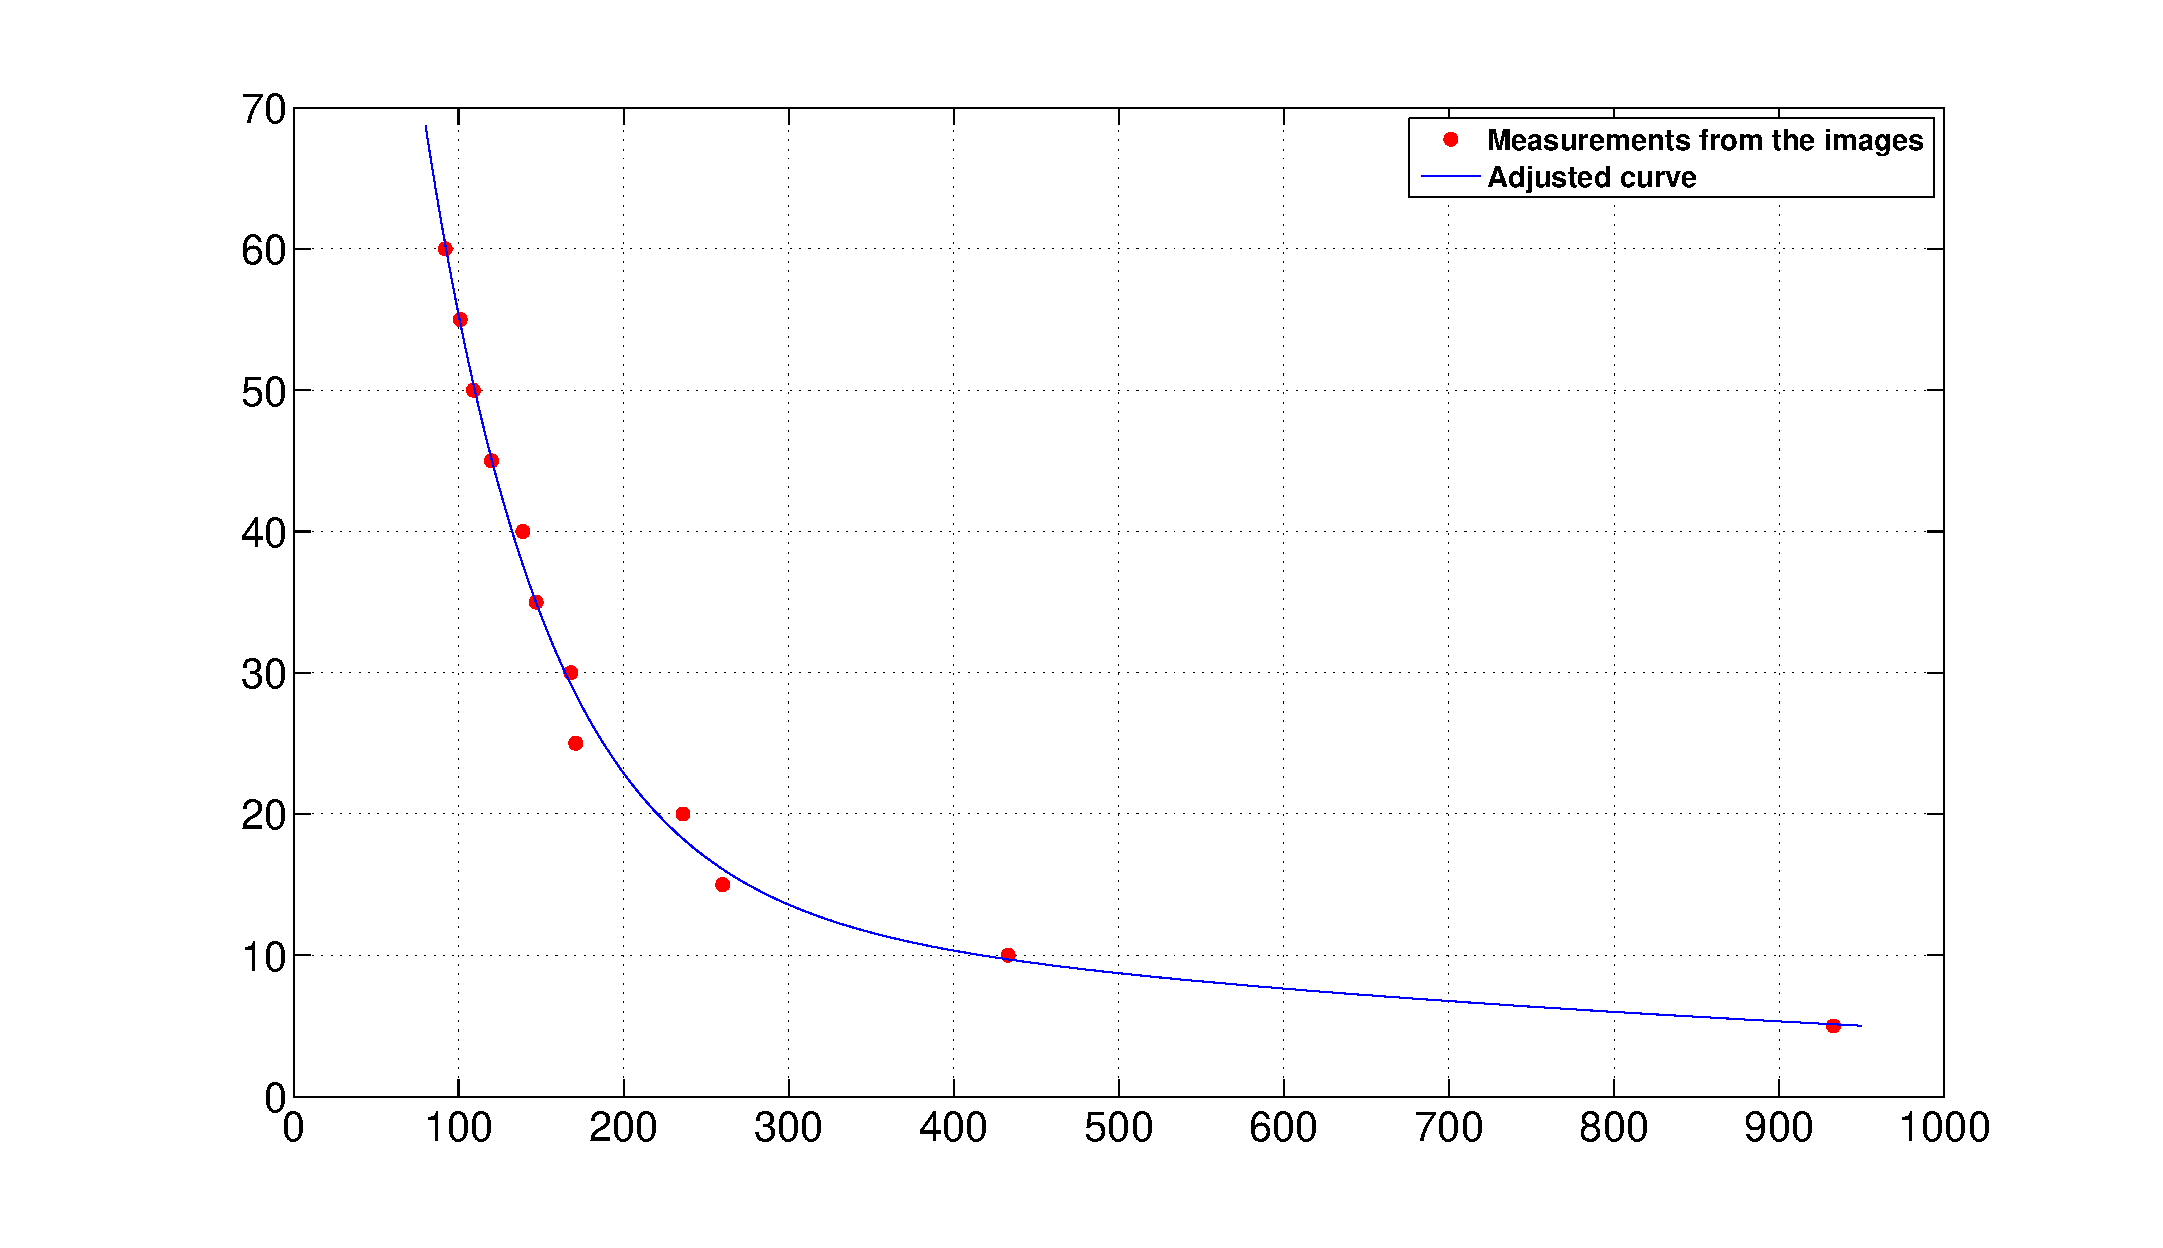
\includegraphics[width=\linewidth]{img/distance_estimation.eps}
\caption{This image shows the curve approximated to the measurements obtained
from the pictures. In the horizontal axis is the width in pixels of
the classification bounding box around the vehicle. In the vertical axis is the
distance in meters to the vehicle. The red points represent the measure obtained
from each image. The blue curve is the predicting model fitted to the data points.}
\label{fig:distance-curve-fitting}
\end{figure} 

It is important to point out that this approximated model is directly related to
the classifier itself. This is because the measurements from the pictures are
obtained through it. This implies that whenever the classifier is changed, a new
coefficients are need to be found.

These coefficients creates a relationship between the width in pixels
of the classified image of the vehicle with the distance in meters to the
vehicle in the real world. Therefore they offer an approximated distance to the
vehicle, giving an initial solution to the problem of distance estimation.

% section Distance estimation (end)
